\documentclass[portuguese]{sbc2025}%

\usepackage[misc,geometry]{ifsym}

\raggedbottom  % Prevent underfull vbox warnings

\usepackage{aas_macros}
\usepackage[bottom]{footmisc}

\usepackage{tabularray}
\usepackage{adjustbox}
\usepackage{stfloats}
\usepackage{placeins}
\usepackage{float}
\usepackage{tikz}
\usetikzlibrary{arrows.meta,positioning,fit,calc,matrix}

\usepackage{afterpage}
\usepackage{url}
\usepackage{pifont}

\setcitestyle{square,comma}

\definecolor{engtitle}{rgb}{0.5,0.5,0.5}
\definecolor{orcidlogo}{rgb}{0.37,0.48,0.13}
\definecolor{unilogo}{rgb}{0.16, 0.26, 0.58}
\definecolor{maillogo}{rgb}{0.58, 0.16, 0.26}
\definecolor{darkblue}{rgb}{0.0,0.0,0.0}
\hypersetup{colorlinks,breaklinks,
            linkcolor=darkblue,urlcolor=darkblue,
            anchorcolor=darkblue,citecolor=darkblue}

\jyear{2025}

\category{Artigo de Pesquisa/Research Paper}
\title[Sistema de Monitoria-IC: Plataforma Web para Gestão de Monitorias Acadêmicas da UFBA]{Sistema de Monitoria-IC: Plataforma Web para Gestão Completa de Monitorias Acadêmicas da UFBA}
\engtitle{\textcolor{engtitle}{Sistema de Monitoria-IC: Web Platform for Complete Management of Academic Monitoring Programs at UFBA}}

\author[Sena et al. 2025]{
\affil{\textbf{Luis Felipe Cordeiro Sena}~\orcidlink{0009-0009-3997-3639}~\textcolor{blue}{\faEnvelopeO}~~[{Universidade Federal da Bahia}~|\href{mailto:luis.sena@ufba.br}{~{\textit{luis.sena@ufba.br}}}~]}

\affil{\textbf{Antoniel Magalhães}~~[{Universidade Federal da Bahia}~| \href{mailto:antoniels@ufba.br}{{\textit{antoniels@ufba.br}}}~]}

\affil{\textbf{João Leahy}~~[{Universidade Federal da Bahia}~| \href{mailto:joao.leahy@ufba.br}{{\textit{joao.leahy@ufba.br}}}~]}

\affil{\textbf{Frederico Araújo Durão}~\orcidlink{0000-0002-7766-6666}~~[{Universidade Federal da Bahia}~| \href{mailto:fdurao@ufba.br}{{\textit{fdurao@ufba.br}}}~]}
}

\begin{document}

\begin{frontmatter}

\maketitle

\begin{mail}
Instituto de Computação, Universidade Federal da Bahia, Av. Milton Santos, s/n - Campus de Ondina, PAF 2, Salvador, BA, 40170-110, Brasil.
\end{mail}

\begin{abstract-pt}
A monitoria acadêmica é um processo fundamental nas universidades brasileiras que permite aos alunos desenvolverem habilidades pedagógicas enquanto auxiliam no processo de ensino-aprendizagem. Porém, o gerenciamento desse processo frequentemente enfrenta desafios relacionados à burocracia, falta de transparência e múltiplos processos manuais ineficientes. Este trabalho apresenta o desenvolvimento do Sistema de Monitoria-IC, uma plataforma Web projetada para automatizar e simplificar o ciclo de vida dos projetos de monitoria na UFBA. A solução proposta digitaliza desde a criação e assinatura de projetos pelos professores até a aprovação administrativa e geração de planilhas consolidadas para envio ao Instituto/PROGRAD. O sistema foi desenvolvido utilizando tecnologias modernas como Next.js 15, TypeScript, tRPC, PostgreSQL e MinIO, seguindo princípios de engenharia de software que garantem escalabilidade e manutenibilidade. A arquitetura implementada separa claramente as responsabilidades entre um Sistema de Processamento de Transações (SPT) para operações cotidianas e funcionalidades gerenciais para análise e controle. A validação técnica através de testes end-to-end demonstra a robustez da solução. Os resultados esperados indicam que a automação proposta tende a eliminar retrabalho administrativo, aumentar a transparência por meio de histórico auditável e estabelecer uma base sólida para a modernização da gestão acadêmica na universidade.
\end{abstract-pt}

\begin{abstract-en}
Academic monitoring is a fundamental process in Brazilian universities that allows students to develop pedagogical skills while assisting in the teaching-learning process. However, managing this process often faces challenges related to bureaucracy, lack of transparency, and multiple inefficient manual procedures. This work presents the development of Sistema de Monitoria-IC, a web platform designed to automate and simplify the lifecycle of monitoring projects at UFBA. The proposed solution digitizes the process from project creation and signing by professors to administrative approval and generation of consolidated spreadsheets for the Institute/PROGRAD. The system was developed using modern technologies such as Next.js 15, TypeScript, tRPC, PostgreSQL, and MinIO, following software engineering principles that ensure scalability and maintainability. The implemented architecture clearly separates responsibilities between a Transaction Processing System (TPS) for daily operations and managerial functionalities for analysis and control. Technical validation through end-to-end tests demonstrates the solution's robustness. Expected results indicate that the proposed automation tends to eliminate administrative rework, increase transparency through auditable history, and establish a solid foundation for modernizing academic management at the university.
\end{abstract-en}

\begin{pchaves}
Gestão Acadêmica, Sistema de Monitoria, Arquitetura de Software, Desenvolvimento Web, Automação de Processos.
\end{pchaves}

\begin{keywords}
Academic Management, Monitoring System, Software Architecture, Web Development, Process Automation.
\end{keywords}

\begin{dates}
% Informações serão preenchidas pelo editor antes da publicação
\end{dates}

\end{frontmatter}

\section{Introdução}
\label{sec:intro}

A monitoria acadêmica representa um dos pilares fundamentais do ensino superior brasileiro, estabelecendo-se como uma prática pedagógica que beneficia simultaneamente monitores, estudantes e docentes. Regulamentada pela Lei nº 9.394/96 (Lei de Diretrizes e Bases da Educação Nacional), a monitoria permite que alunos com destacado desempenho acadêmico auxiliem seus pares no processo de aprendizagem, desenvolvendo competências didáticas enquanto aprofundam seus conhecimentos na disciplina \cite{Brasil1996}.

Na Universidade Federal da Bahia (UFBA), o programa de monitoria segue um fluxo complexo que envolve múltiplos atores e etapas interdependentes. O processo inicia-se com o planejamento semestral, quando a administração importa dados de disciplinas e professores. Em seguida, os docentes criam e submetem projetos de monitoria que precisam ser aprovados administrativamente. Após a aprovação, ocorre a publicação de editais internos, inscrição de candidatos, processo seletivo, alocação de bolsas, e finalmente, a consolidação de dados para envio à PROGRAD (Pró-Reitoria de Graduação).

A literatura de Sistemas de Informação fornece evidências de que a digitalização e a automação de processos reduzem custos transacionais, eliminam retrabalho e aumentam a confiabilidade e a auditabilidade dos registros \cite{Laudon_Laudon_2011, Davenport1993, Hammer1993}. Em contextos públicos e acadêmicos, iniciativas de governo digital e transformação digital têm sido associadas a ganhos de eficiência administrativa e transparência, desde que apoiadas por arquitetura tecnológica moderna e governança de dados adequada \cite{WorldBank2022, UNESCO2023}. No escopo deste trabalho, tais fundamentos são adotados para sustentar a proposta de um sistema unificado de monitoria, substituindo fluxos fragmentados por um \textit{workflow} padronizado, rastreável e escalável.

Apesar de sua importância reconhecida, a gestão dos programas de monitoria na UFBA ainda depende predominantemente de processos manuais e fragmentados. Formulários em papel, planilhas eletrônicas dispersas, comunicação via e-mail e ausência de um sistema centralizado caracterizam o cenário atual, resultando em ineficiências operacionais significativas. Essa realidade contrasta com a tendência global de digitalização e automação de processos administrativos no ambiente acadêmico. \citet{Laudon_Laudon_2011} argumentam que a tecnologia da informação constitui uma das principais ferramentas para alcançar excelência operacional.

\subsection{Identificação do Problema}

O processo de monitoria na UFBA é lento, caro e opaco. Do lado docente, há retrabalho sistemático (recriação de projetos a cada semestre), dispersão de documentos (planilhas, PDFs e e-mails) e ausência de trilhas de auditoria --- combinação que consome horas de atividades-fim e eleva o risco de erro. A seleção permanece predominantemente manual e heterogênea entre departamentos, impedindo comparabilidade de critérios e produzindo falhas de registro.

Para estudantes, a descoberta de vagas é imprevisível e a jornada é fragmentada: múltiplos formulários, anexos por canais distintos e ausência de um painel único para acompanhar prazos, status e resultados --- o que reforça a percepção de opacidade e desestimula a participação.

Administrativamente, a consolidação de dados heterogêneos gera retrabalho, dificulta a conformidade com regulamentos e prazos e fragiliza a prestação de contas. Sem um repositório transacional e analítico integrado, relatórios custam caro e análises históricas confiáveis tornam-se inviáveis para decisões como distribuição de bolsas e avaliação de efetividade de projetos.

Em síntese, há uma lacuna tecnológica clara: falta um sistema de informação \textit{fim-a-fim} específico para monitoria que integre criação e aprovação de projetos, publicação de editais, inscrições, seleção, aceite de vagas e consolidações finais. A literatura indica que a automação e a padronização, apoiadas por arquitetura adequada e governança de dados, reduzem custos transacionais, retrabalho e erros e elevam a confiabilidade e a auditabilidade dos registros \cite{Davenport1993, Hammer1993, Laudon_Laudon_2011, WorldBank2022, UNESCO2023}.

\subsection{Objetivos}

Este trabalho documenta o desenvolvimento e implementação do Sistema de Monitoria-IC, uma plataforma Web completa para gestão dos projetos de monitoria do Instituto de Computação da UFBA. O objetivo central é substituir fluxos manuais e dispersos por um sistema único que garanta transparência, rastreabilidade e padronização de todo o processo de monitoria.

Os objetivos específicos incluem:

\begin{enumerate}
  \item Digitalizar o ciclo completo de projetos de monitoria: desde a criação com templates reutilizáveis, assinatura digital pelo professor, submissão, até aprovação administrativa e publicação de editais

  \item Automatizar o processo seletivo: permitindo inscrições online, captura automática de notas e CR do histórico, consideração de equivalências entre disciplinas, e publicação transparente de resultados

  \item Sistematizar a alocação de bolsas: com geração automática de planilhas para o Instituto, configuração do total de bolsas informado pela PROGRAD, e alocação por projeto com validações automáticas

  \item Eliminar trabalhos manuais repetitivos: através de automação de notificações por e-mail, geração de documentos PDF, e integração com armazenamento de arquivos

  \item Fornecer base analítica para tomada de decisões: com dashboards administrativos, APIs para integração, e relatórios consolidados para análises institucionais
\end{enumerate}

\subsection{Fora do Escopo}

Embora o sistema cubra o ciclo de vida completo da monitoria acadêmica, algumas funcionalidades foram deliberadamente excluídas do escopo deste trabalho. Primeiro, o módulo de relatórios finais e certificados (Fase 6 do fluxo de monitoria) foi especificado nos requisitos mas não implementado, sendo priorizado como trabalho futuro devido a restrições de tempo e à necessidade de validação do fluxo principal antes de sua expansão. Segundo, a integração automática com o sistema acadêmico institucional (SIAC ou SIGAA) para captura de históricos e notas permanece manual, exigindo que estudantes anexem documentos comprobatórios durante a inscrição. Terceiro, o sistema foi desenvolvido especificamente para o Instituto de Computação da UFBA, com adaptações necessárias para expansão a outros departamentos ou instituições. Quarto, funcionalidades de analytics avançado, como sistema de recomendação para correspondência entre aluno e projeto ou predição de desempenho com técnicas de aprendizado de máquina, foram identificadas como melhorias futuras mas não integradas nesta versão inicial. Por fim, um aplicativo móvel nativo não foi desenvolvido, embora a interface Web seja responsiva e funcione adequadamente em dispositivos móveis via navegador.

\subsection{Contribuições}

Este trabalho apresenta quatro contribuições principais para a área de Sistemas de Informação aplicados à gestão acadêmica. Primeira, propõe e implementa uma arquitetura em três camadas (Router-Service-Repository) específica para o domínio de monitoria acadêmica, demonstrando como separar responsabilidades entre apresentação, lógica de negócio e acesso a dados em um sistema transacional com múltiplos atores e requisitos formais de auditoria. Segunda, desenvolve um workflow automatizado completo que cobre as cinco primeiras fases do ciclo de monitoria (planejamento, aprovação, alocação, seleção e consolidação), incluindo funcionalidades inovadoras como templates reutilizáveis de projetos, assinaturas digitais integradas, consideração automática de equivalências curriculares e geração de documentos formais em PDF, resultando em significativa redução no tempo gasto em tarefas administrativas repetitivas. Terceira, documenta um estudo de caso real de transformação digital em instituição pública brasileira, fornecendo evidências técnicas (57 testes automatizados com 100\% de aprovação) e organizacionais (análise do estado da prática em dez universidades públicas) que podem orientar iniciativas similares em outras instituições de ensino superior. Quarta, disponibiliza uma solução de código aberto baseada em tecnologias modernas (Next.js 15, tRPC v11, PostgreSQL, TypeScript) com documentação técnica completa, permitindo replicação, adaptação e extensão por outras universidades que enfrentem desafios similares na gestão de programas de monitoria.

\subsection{Estrutura do Trabalho}

Este artigo está organizado da seguinte forma: a Seção 2 apresenta os fundamentos teóricos sobre Sistemas de Informação e monitoria acadêmica. A Seção 3 analisa trabalhos relacionados e o estado da prática em universidades brasileiras. A Seção 4 detalha o Sistema de Monitoria-IC, iniciando pela metodologia de desenvolvimento adotada (4.1), seguida pelos requisitos funcionais e não-funcionais (4.2), arquitetura em camadas (4.3), modelo de dados normalizado (4.4), fluxo de processos do ciclo completo de monitoria (4.5), stack tecnológico implementado (4.6) e interfaces especializadas por perfil de usuário (4.7). A Seção 5 apresenta a avaliação experimental, incluindo metodologia de testes, resultados técnicos obtidos e limitações identificadas. Por fim, a Seção 6 conclui o trabalho e aponta direções futuras.

\section{Fundamentação Teórica}
\label{sec:background}

\subsection{Monitoria Acadêmica}

A monitoria acadêmica constitui uma modalidade de ensino-aprendizagem que contribui para a formação integrada do aluno nas atividades de ensino, pesquisa e extensão dos cursos de graduação. Conforme estabelecido pela Lei de Diretrizes e Bases da Educação Nacional (Lei nº 9.394/96), as universidades devem aproveitar estudantes de bom rendimento acadêmico em tarefas de ensino e pesquisa \cite{Brasil1996}.

O processo de monitoria na UFBA segue diretrizes institucionais que estabelecem critérios de seleção baseados no desempenho acadêmico (nota na disciplina e Coeficiente de Rendimento), definem modalidades de participação (bolsista e voluntário), delimitam responsabilidades de monitores, professores e coordenação, regulam o fluxo de aprovação de projetos e alocação de recursos e definem requisitos de certificação ao final do período.

Estudos sobre programas de monitoria demonstram benefícios significativos: desenvolvimento de habilidades didáticas nos monitores \cite{Natario2010}, melhoria no desempenho acadêmico dos estudantes assistidos \cite{Frison2016}, e apoio essencial aos docentes na condução de atividades práticas \cite{Dantas2014}. Entretanto, esses mesmos estudos apontam desafios na gestão administrativa desses programas, especialmente relacionados à burocracia e falta de ferramentas adequadas.

\subsection{Sistemas de Informação na Gestão Acadêmica}

Sistemas de Processamento de Transações (SPTs) são “sistemas informatizados que realizam e registram as transações rotineiras necessárias ao funcionamento organizacional” \cite{Laudon_Laudon_2011}. No contexto acadêmico, gerenciam operações como matrículas, lançamento de notas, controle de frequência e, neste trabalho, o ciclo de vida de projetos de monitoria. Suas características essenciais incluem alta precisão e confiabilidade dos dados, processamento eficiente de grandes volumes transacionais, mecanismos de auditoria e rastreabilidade e alta disponibilidade para sustentar operações críticas.

Já os Sistemas de Informações Gerenciais (SIG) “resumem e relatam as operações básicas da organização usando dados fornecidos pelos SPTs” \cite{Laudon_Laudon_2011}. No Sistema de Monitoria-IC, o componente gerencial materializa-se em painéis e relatórios consolidados para acompanhar o andamento dos processos, analisar tendências históricas, auxiliar a distribuição de recursos e gerar documentos formais para órgãos superiores.

A separação de responsabilidades entre SPT (camada operacional) e SIG (camada analítica) fundamenta a arquitetura do Sistema de Monitoria-IC. O SPT gerencia o ciclo de vida de cada transação — cadastros, aprovações, inscrições — enquanto o SIG consome registros consolidados para análises e relatórios. Essa divisão favorece escalabilidade independente, facilita manutenção e evolução, reduz acoplamento entre operações e análises e permite otimizações específicas de desempenho em cada camada.

% Subsecção 2.3 (Tecnologias) removida; conteúdo consolidado na Seção 4 (Implementação e Tecnologias)

\section{Trabalhos Relacionados}
\label{sec:related-work}

% Subsecção 3.1 removida conforme orientação

\subsection{Levantamento do Estado da Prática}

Para avaliar o estado atual da gestão de monitoria em universidades brasileiras, foi realizado um levantamento documental nos cursos de Computação das dez universidades públicas mais bem classificadas segundo o Ranking Universitário Folha (RUF) 2024 \cite{folha2024ruf}. A análise concentrou-se em fontes públicas: páginas institucionais dos sistemas acadêmicos, editais de monitoria e documentos de orientação disponíveis em 2024--2025. Não houve acesso a sistemas internos autenticados, o que impõe limites importantes à generalização dos resultados. A Tabela~\ref{tab:estado-pratica} sintetiza os resultados desse levantamento.

\begin{table*}[htb]
  \centering
\caption{Panorama sintético da gestão de monitoria em universidades públicas brasileiras, a partir de fontes públicas (sítios institucionais e editais).\\Fonte: páginas oficiais dos sistemas Júpiter/USP \cite{USPJupiter}, SIGA/UFRJ \cite{UFRJ_SIGA}, SIGAA/UnB \cite{UnB_SIGAA}, CAGR/UFSC \cite{UFSC_CAGR} e SEI/UNIFESP \cite{UNIFESP_SEI}, complementadas por editais e orientações públicas (2024--2025).}
  \label{tab:estado-pratica}
  \begin{adjustbox}{max width=\textwidth}
    \begin{tabular}{|l|c|p{3.5cm}|p{6cm}|}
      \hline
      \textbf{Universidade} & \textbf{Uso de sistema acadêmico} & \textbf{Evidências de ferramentas} & \textbf{Observações a partir das fontes públicas} \\
      \hline
      USP     & Sim    & Júpiter + formulários complementares & Monitoria relacionada ao sistema acadêmico geral, com seleção apoiada em formulários e orientações departamentais. \\
      \hline
      Unicamp & Parcial & Páginas do PAD e editais locais     & Documentação pública menciona critérios e programas (por exemplo, PAD), mas não detalha mecanismo único e integrado de inscrição para todos os cursos. \\
      \hline
      UFRGS   & Sim    & Portal do Aluno                      & Portal acadêmico institucional com funcionalidades para atividades acadêmicas; editais indicam processos complementares por unidade. \\
      \hline
      UFRJ    & Sim    & SIGA + documentos administrativos    & Parte do cadastro ocorre no SIGA; editais descrevem etapas adicionais conduzidas por departamentos e comissões. \\
      \hline
      UFMG    & Parcial & Editais e formulários online         & Editais indicam uso de formulários eletrônicos simples para inscrição, com consolidações posteriores em planilhas e documentos administrativos. \\
      \hline
      UNESP   & Parcial & Editais + documentação interna       & Não foram localizados, nas fontes públicas, módulos específicos de monitoria; editais sugerem trâmites administrativos distribuídos entre unidades. \\
      \hline
      UFSC    & Sim    & CAGR                                 & Sistema acadêmico com módulo genérico; as especificidades da monitoria são tratadas em editais e orientações complementares. \\
      \hline
      UnB     & Sim    & SIGAA                                & SIGAA oferece módulo para atividades acadêmicas; editais indicam que a monitoria utiliza esse módulo em combinação com procedimentos departamentais. \\
      \hline
      UNIFESP & Parcial & SEI + formulários                    & Processos administrativos tramitam via SEI, com inscrições tipicamente apoiadas em formulários e documentos anexos. \\
      \hline
      UFPR    & Parcial & Editais + formulários online         & Editais recentes mencionam uso de formulários (como Google/Microsoft Forms) e trâmites eletrônicos departamentais, sem referência a módulo dedicado de monitoria. \\
      \hline
    \end{tabular}
  \end{adjustbox}
\end{table*}

Com base nesse levantamento, não foi possível confirmar a existência de um sistema específico e completo de monitoria em nenhuma das instituições analisadas apenas a partir de fontes públicas. Em vários casos, há evidência de sistemas acadêmicos consolidados (como Júpiter, SIGA, SIGAA e CAGR) que oferecem algum suporte ao processo, mas as descrições dos editais e das orientações complementares indicam que etapas críticas --- como submissão de projetos, consolidação de inscrições, definição de bolsas e emissão de relatórios --- permanecem distribuídas entre formulários eletrônicos genéricos, documentos administrativos e fluxos manuais conduzidos por departamentos.

Outro padrão observado é a fragmentação dos canais de interação: o estudante frequentemente acessa uma combinação de páginas institucionais, formulários externos e comunicados por e-mail para compreender o processo de monitoria, enquanto professores e coordenações dependem de planilhas, documentos anexados em sistemas de processo eletrônico e rotinas internas de consolidação. Mesmo nos casos em que há módulos de ``atividades acadêmicas'' ou programas de apoio didático, a documentação pública não descreve workflows fim-a-fim de monitoria equivalentes ao ciclo completo apresentado na Seção~\ref{sec:system}.

Essas limitações metodológicas são importantes: o levantamento baseia-se apenas em evidências disponíveis publicamente, em um recorte temporal específico (2024--2025) e focado nos cursos de Computação. É possível que existam soluções internas não documentadas, iniciativas departamentais em fase piloto ou sistemas legados de uso restrito que não foram capturados nessa análise. Ainda assim, o panorama obtido é consistente com a literatura sobre transformação digital na gestão acadêmica \cite{Laudon_Laudon_2011, Davenport1993, Hammer1993, WorldBank2022, UNESCO2023}, que aponta para a coexistência de sistemas institucionais robustos com processos específicos de alto teor manual e fragmentado.

À luz desse cenário, o Sistema de Monitoria-IC distingue-se por cinco dimensões principais. Primeiro, é específico para o workflow de monitoria, ao invés de reutilizar módulos genéricos concebidos para múltiplos processos acadêmicos. Segundo, cobre as etapas centrais do ciclo de vida, desde a criação e aprovação de projetos até a consolidação final para a PROGRAD, reduzindo a fragmentação observada nas instituições analisadas. Terceiro, automatiza etapas críticas via integrações com armazenamento de arquivos, geração de PDFs, assinaturas digitais e notificações, diminuindo significativamente a necessidade de retrabalho manual. Quarto, adota um stack tecnológico moderno (Next.js 15, tRPC v11, PostgreSQL, MinIO) com foco em experiência do usuário, \textit{type-safety} e desempenho, em contraste com soluções frequentemente baseadas em sistemas legados e formulários genéricos. Por fim, garante transparência e rastreabilidade através de histórico auditável e acesso diferenciado por papéis (admin, professor, aluno, chefe de departamento), alinhando-se às recomendações de boas práticas em governo digital e governança de dados em educação superior.

\subsection{Projetos Correlatos no Instituto de Computação}

No contexto do próprio Instituto de Computação da UFBA, há Trabalhos de Conclusão de Curso recentes que tratam de sistemas Web para automatização de processos acadêmico-administrativos, oferecendo um referencial importante para situar o Sistema de Monitoria-IC. O trabalho ``IC-Requests: um sistema sensível ao contexto para suporte a solicitações acadêmicas'', de \citet{machado2024icrequests}, propõe um sistema Web para gerenciar requerimentos acadêmicos de alunos do IC-UFBA. Em termos de escopo, o IC-Requests foca em um processo mais delimitado --- solicitações específicas como trancamentos, declarações e ajustes de matrícula --- enquanto o Sistema de Monitoria-IC cobre o ciclo de vida completo da monitoria acadêmica, desde a criação de projetos pelos docentes até a emissão de relatórios finais e consolidação para a PROGRAD. Metodologicamente, o IC-Requests dá ênfase à avaliação empírica com usuários, incluindo questionários de usabilidade com alunos, ao passo que o Monitoria-IC privilegia o detalhamento arquitetural e a robustez técnica, com testes automatizados cobrindo o fluxo transacional. As duas abordagens são complementares: o IC-Requests contribui com uma validação centrada no usuário, e o Sistema de Monitoria-IC aprofunda a engenharia de software em um domínio mais amplo e complexo.

Outro projeto relevante é ``AlertUFBA: um sistema Web de orientações sobre segurança e emergência no contexto universitário'', de \citet{santos2023alertufba}, que desenvolve uma plataforma informativa para centralizar orientações em caso de emergências no campus. Embora o domínio seja distinto do da monitoria, há semelhanças metodológicas na condução de entrevistas e questionários com usuários para validar a utilidade do sistema. Em comparação, o AlertUFBA atua sobretudo como um canal de comunicação e prevenção, enquanto o Sistema de Monitoria-IC implementa um fluxo transacional estruturado, com múltiplos atores e requisitos formais de prestação de contas institucional. Assim, o Monitoria-IC posiciona-se mais próximo de um Sistema de Processamento de Transações (SPT) integrado a funcionalidades gerenciais, conforme discutido na Seção~\ref{sec:background}. Em síntese, ambos os trabalhos do IC-UFBA contribuem metodologicamente com avaliação de usabilidade e validação empírica, enquanto o Sistema de Monitoria-IC se diferencia pelo escopo mais abrangente (ciclo completo de monitoria versus processos específicos), pela arquitetura robusta em três camadas (Router-Service-Repository) e pela natureza transacional com múltiplos atores interdependentes, caracterizando um sistema de informação empresarial completo ao invés de soluções pontuais ou informativas.

\subsection{Comparação com Sistemas Acadêmicos Existentes}

Além dos trabalhos de TCC, diversas universidades brasileiras utilizam sistemas acadêmicos integrados, como JúpiterWeb (USP), SIGA (UFRJ), SIGAA (UnB), CAGR (UFSC) e SEI (UNIFESP), que oferecem módulos genéricos para gestão de disciplinas, matrículas e processos administrativos. A análise documental realizada para este trabalho, baseada em páginas institucionais e editais públicos, não identificou, entretanto, um módulo específico e completo de monitoria acadêmica que cubra de forma integrada todas as etapas descritas na Seção~\ref{sec:system}. A Tabela~\ref{tab:comparacao-sistemas} resume, de forma sintética, o posicionamento do Sistema de Monitoria-IC em relação a esses sistemas genéricos, evidenciando as diferenças de escopo, suporte à monitoria e avaliação documentada.

\begin{table*}[htb]
  \centering
  \caption{Comparação sintética entre sistemas acadêmicos genéricos e o Sistema de Monitoria-IC.}
  \label{tab:comparacao-sistemas}
  \begin{adjustbox}{max width=\textwidth}
    \begin{tabular}{|l|p{3cm}|p{3.5cm}|p{4cm}|p{3.5cm}|}
      \hline
      \textbf{Sistema} & \textbf{Escopo principal} & \textbf{Suporte à monitoria} & \textbf{Workflow de monitoria fim-a-fim} & \textbf{Avaliação com usuários (nas fontes públicas)} \\
      \hline
      JúpiterWeb (USP) & Gestão acadêmica geral (grades, matrículas, histórico) & Mencionado em editais e orientações complementares, sem módulo dedicado descrito publicamente & Não identificado em fontes públicas; etapas de monitoria aparentam depender de formulários e fluxos departamentais & Não documentada explicitamente \\
      \hline
      SIGA (UFRJ) & Sistema integrado de gestão acadêmica & Utilizado em combinação com documentos administrativos e comissões departamentais para monitoria & Não identificado módulo específico que integre todas as fases da monitoria & Não documentada explicitamente \\
      \hline
      SIGAA (UnB) & Gestão de atividades acadêmicas e administrativas & Oferece suporte a atividades acadêmicas em geral; a monitoria é tratada em conjunto com procedimentos departamentais & Não há descrição pública de um workflow completo de monitoria como o proposto neste trabalho & Não documentada explicitamente \\
      \hline
      CAGR (UFSC) & Controle acadêmico da graduação & Possui funcionalidades de apoio; monitoria complementada por editais e orientações externas ao sistema & Não identificado módulo fim-a-fim de monitoria com automação de relatórios e consolidação & Não documentada explicitamente \\
      \hline
      SEI (UNIFESP) & Tramitação eletrônica de processos & Utilizado para gestão de documentos administrativos, incluindo etapas de monitoria & Focado em processos administrativos; o fluxo de monitoria depende de formulários e anexos geridos pelos departamentos & Não documentada explicitamente \\
      \hline
      Sistema de Monitoria-IC & Workflow completo de monitoria (projetos, bolsas, inscrições, seleção, consolidação) & Módulo específico para monitoria, concebido para o contexto da UFBA & Parcial: cobre integralmente as fases 1 a 5; relatórios/certificados foram especificados como evolução & Avaliação técnica por testes automatizados; avaliação com usuários prevista como trabalho futuro \\
      \hline
    \end{tabular}
  \end{adjustbox}
\end{table*}

À luz dessa comparação, o Sistema de Monitoria-IC distingue-se por ser um sistema específico para monitoria acadêmica, cobrindo o ciclo de vida completo do processo e integrando funcionalidades transacionais e gerenciais em uma única plataforma. A solução proposta não pretende substituir sistemas acadêmicos institucionais existentes, mas sim complementar a infraestrutura da UFBA com um módulo especializado, passível de integração futura com sistemas como SIAC ou SIGAA.

\section{Sistema de Monitoria-IC}
\label{sec:system}

\subsection{Metodologia e Requisitos}
\label{sec:methodology}

O desenvolvimento seguiu metodologia estruturada com quatro fases: análise de requisitos (entrevistas com coordenadores e análise de editais 2019-2023), design arquitetural (camadas com separação de responsabilidades e \textit{type-safety} via TypeScript/tRPC), implementação ágil em ciclos de duas semanas organizada por domínios (projetos, editais, inscrições, seleção), e validação técnica com testes automatizados (55 testes unitários/integração, E2E com Playwright).

Os principais requisitos funcionais incluem: importação de planejamento semestral com validação SIAPE, templates reutilizáveis entre semestres, workflow de aprovação com estados (DRAFT/SUBMITTED/APPROVED/REJECTED), assinatura digital de projetos, alocação de bolsas com validação de limites, publicação de editais, portal de inscrições com upload de documentos, seleção com equivalências de disciplinas, e geração de planilhas consolidadas para PROGRAD. Requisitos não-funcionais contemplam desempenho (latência API <100ms, carregamento <3s), segurança (RBAC, validação Zod, Lucia Auth), e confiabilidade (disponibilidade >99\%, backups incrementais).

\subsection{Arquitetura}

O Sistema de Monitoria-IC foi projetado seguindo uma arquitetura em camadas que separa claramente as responsabilidades e promove manutenibilidade e escalabilidade, conforme ilustrado na Figura \ref{fig:architecture}. A arquitetura segue o padrão de três camadas com componentes especializados. Na implementação prática, as camadas de Apresentação (cliente React) e Aplicação (rotas tRPC) coexistem na mesma aplicação Next.js (padrão full-stack monolítico), enquanto a separação lógica em quatro camadas apresentada facilita a compreensão didática das responsabilidades de cada componente arquitetural.

A \textbf{camada de apresentação} utiliza Next.js 15 com React e TypeScript, oferecendo interfaces especializadas por perfil. Componentes shadcn/ui e Tailwind CSS garantem consistência visual, enquanto React Hook Form com Zod implementa validação compartilhada cliente-servidor. React Query gerencia cache e sincronização de estado.

A \textbf{camada de aplicação} expõe a API via tRPC v11, garantindo \textit{type-safety} fim-a-fim. Lucia Auth gerencia autenticação com sessões seguras, e o sistema RBAC controla permissões por papel (admin, professor, aluno, chefe de departamento).

A \textbf{camada de negócio} concentra serviços especializados: \texttt{ProjectService} (ciclo de vida de projetos), \texttt{SelectionService} (inscrições e seleção com equivalências), \texttt{NotificationService} (e-mails automáticos), \texttt{DocumentService} (PDFs e assinaturas digitais) e \texttt{AnalyticsService} (dashboards e relatórios).

A \textbf{camada de dados} utiliza PostgreSQL com Drizzle ORM para consultas tipadas, MinIO para armazenamento de arquivos (compatível S3), e Nodemailer para envio de e-mails via SMTP institucional. Backups incrementais são realizados a cada 6 horas.

\begin{figure}[t]
  \centering
  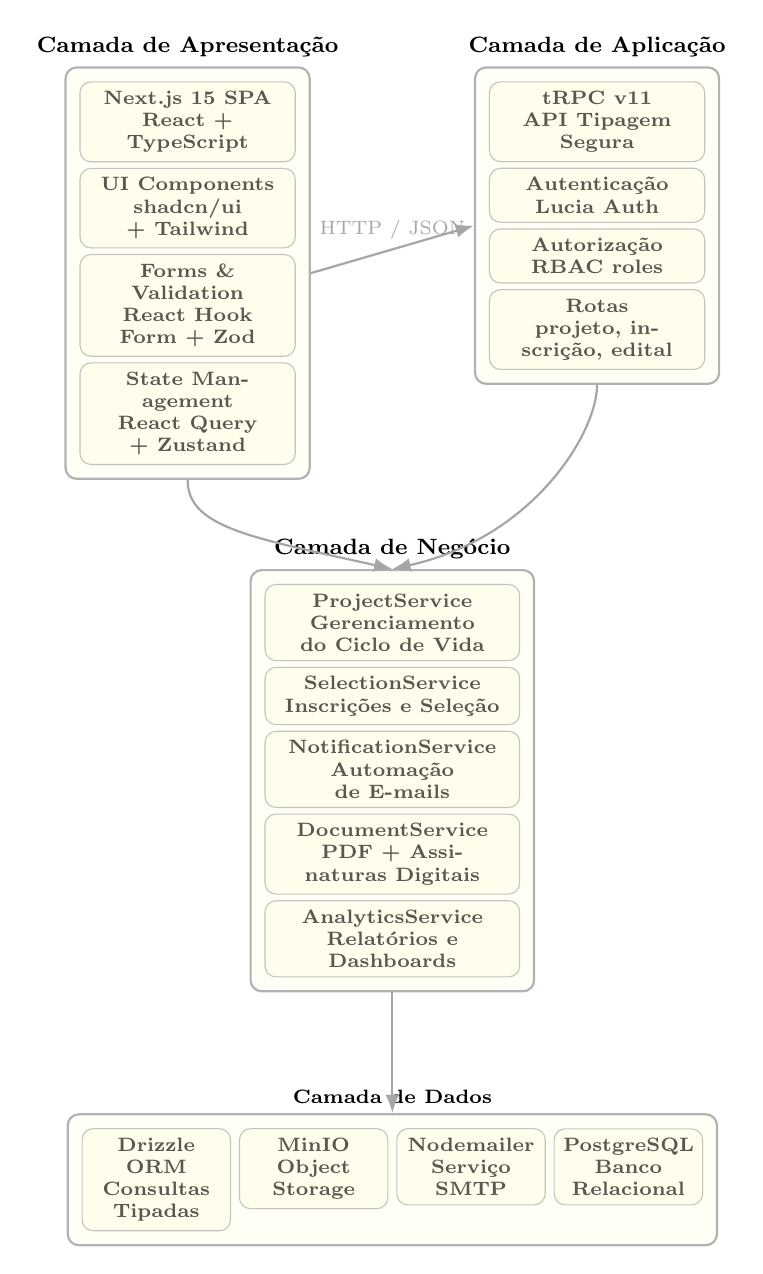
\begin{tikzpicture}[
    layer/.style={rounded corners, draw=gray!60, fill=yellow!10, fill opacity=0.35, draw opacity=1, thick, inner sep=5pt},
    box/.style={draw=gray!70, rounded corners, fill=yellow!6, text width=2.5cm, align=center, minimum height=0.6cm, font=\scriptsize\bfseries, text=black},
    smallbox/.style={draw=gray!70, rounded corners, fill=yellow!6, text width=3.0cm, align=center, minimum height=0.6cm, font=\scriptsize\bfseries, text=black},
    databox/.style={draw=gray!70, rounded corners, fill=yellow!6, text width=1.65cm, align=center, minimum height=0.55cm, font=\scriptsize\bfseries, text=black},
    connector/.style={-Latex, thick, gray!70}
  ]
    % Camada de Apresentação
    \matrix (presentation) [
      matrix of nodes,
      nodes={box},
      row sep=2pt,
      column sep=0pt,
      matrix anchor=north,
      anchor=north
    ] at (-2.6,0) {
      {Next.js 15 SPA\\React + TypeScript} \\
      {UI Components\\shadcn/ui + Tailwind} \\
      {Forms \& Validation\\React Hook Form + Zod} \\
      {State Management\\React Query + Zustand} \\
    };
    \node[layer, fit=(presentation-1-1)(presentation-4-1), label={[font=\footnotesize\bfseries]above:Camada de Apresentação}] (presentationLayer) {};

    % Camada de Aplicação
    \matrix (application) [
      matrix of nodes,
      nodes={box},
      row sep=2pt,
      column sep=0pt,
      matrix anchor=north,
      anchor=north
    ] at (2.6,0) {
      {tRPC v11\\API Tipagem Segura} \\
      {Autenticação\\Lucia Auth} \\
      {Autorização\\RBAC roles} \\
      {Rotas\\projeto, inscrição, edital} \\
    };
    \node[layer, fit=(application-1-1)(application-4-1), label={[font=\footnotesize\bfseries]above:Camada de Aplicação}] (applicationLayer) {};

    % Camada de Negócio
    \coordinate (topMid) at ($(presentationLayer.south)!0.5!(applicationLayer.south)$);
    \matrix (business) [
      matrix of nodes,
      nodes={smallbox},
      row sep=2pt,
      column sep=0pt,
      matrix anchor=north,
      anchor=north
    ] at ($(topMid)+(0,-1.8)$) {
      {ProjectService\\Gerenciamento do Ciclo de Vida} \\
      {SelectionService\\Inscrições e Seleção} \\
      {NotificationService\\Automação de E-mails} \\
      {DocumentService\\PDF + Assinaturas Digitais} \\
      {AnalyticsService\\Relatórios e Dashboards} \\
    };
    \node[layer, fit=(business-1-1)(business-5-1), label={[font=\footnotesize\bfseries]above:Camada de Negócio}] (businessLayer) {};

    % Camada de Dados
    \matrix (data) [
      matrix of nodes,
      nodes={databox},
      row sep=0pt,
      column sep=0.1cm,
      matrix anchor=north,
      anchor=north
    ] at ($(businessLayer.south)+(0,-1.6)$) {
      {Drizzle ORM\\Consultas Tipadas} &
      {MinIO\\Object Storage} &
      {Nodemailer\\Serviço SMTP} &
      {PostgreSQL\\Banco Relacional} \\
    };
    \node[layer, fit=(data-1-1)(data-1-4), label={[font=\scriptsize\bfseries]above:Camada de Dados}] (dataLayer) {};

    % Conectores
    \draw[connector] (presentationLayer.east) -- node[above,font=\scriptsize]{HTTP / JSON} (applicationLayer.west);
    \draw[connector] (presentationLayer.south) .. controls +(0,-0.6) and +(-1.8,0.4) .. (businessLayer.north);
    \draw[connector] (applicationLayer.south) .. controls +(0,-0.6) and +(1.8,0.4) .. (businessLayer.north);
    \draw[connector] (businessLayer.south) -- (dataLayer.north);
  \end{tikzpicture}
  \caption{Arquitetura lógica do Sistema de Monitoria-IC.}
  \label{fig:architecture}
\end{figure}

O sistema oferece interfaces especializadas para cada perfil: \textbf{administradores} acessam dashboard com métricas, gerenciamento de projetos, editais, alocação de bolsas e geração de planilhas PROGRAD; \textbf{professores} criam/editam projetos com templates reutilizáveis, realizam assinatura digital e conduzem o processo seletivo; \textbf{estudantes} consultam vagas disponíveis, realizam inscrições com upload de documentos e acompanham resultados. O sistema implementa validação Zod em cliente e servidor, comunicação HTTPS e minimização de dados conforme LGPD.

\subsection{Modelo de Dados}

O modelo de dados segue princípios de normalização (3NF) e integridade referencial. As principais entidades incluem: \texttt{user} (autenticação e perfil), estendida por \texttt{professor} e \texttt{aluno}; hierarquia acadêmica (\texttt{departamento}, \texttt{curso}, \texttt{disciplina}); e domínio de monitoria (\texttt{projeto}, \texttt{inscricao}, \texttt{vaga}, \texttt{edital}). A Figura \ref{fig:data-model} apresenta o diagrama entidade-relacionamento resumido.

\begin{figure}[p]
  \centering
  \includegraphics[width=\linewidth,keepaspectratio]{images/monitoria/data-model-erd.png}
  \caption{Modelo de dados resumido do domínio de monitoria.}
  \label{fig:data-model}
\end{figure}

\subsection{Fluxo de Processos}

O fluxo de monitoria é orquestrado em cinco etapas contínuas que estruturam o semestre, conforme ilustrado na Figura \ref{fig:process-flow}. Neste trabalho, a etapa enfatizada (e adotada como foco da validação do sistema) é o fluxo de \textit{Planejamento \& Criação} até \textit{Aprovação \& PROGRAD}, pois concentra o maior impacto na redução de retrabalho e na padronização dos documentos encaminhados ao Instituto. Na prática, esse fluxo se materializa em módulos específicos da aplicação: (i) a administração acessa \textit{Importar Planejamento} para enviar a planilha semestral; o sistema valida o arquivo, cria projetos iniciais por disciplina e dispara notificações automáticas aos professores, sinalizando que há projetos pendentes de revisão e assinatura; (ii) ao acessar o dashboard, o professor visualiza os projetos em estado de pendência e, caso não exista template prévio, é conduzido a criar um template padrão da disciplina (título, descrição, carga horária e atividades), permitindo reuso nos próximos semestres; (iii) em seguida, o professor revisa o projeto do semestre, gera o PDF e realiza a assinatura digital no módulo \textit{Assinatura de Documentos}; (iv) a submissão assinada torna o projeto elegível para revisão administrativa em \textit{Gerenciar Projetos}, onde o administrador pode aprovar ou rejeitar com feedback; e (v) quando aprovado, o projeto passa a compor automaticamente a planilha consolidada em \textit{Planilha para Instituto}, disponível para download e envio por e-mail, incluindo referências e anexos aos PDFs dos projetos aprovados, facilitando o trâmite com o Instituto/PROGRAD.

As demais etapas (\textit{Alocação \& Edital}, \textit{Inscrições \& Seleção} e \textit{Aceite \& Consolidação}) complementam o ciclo e já estão contempladas no sistema, permitindo a configuração de vagas, publicação de edital interno, inscrição de estudantes, seleção e consolidação final de dados bancários e planilhas para órgãos responsáveis.\footnote{O recorte deste trabalho segue o planejamento visível na Figura 3, com foco nas fases implementadas até a geração da planilha consolidada para o Instituto/PROGRAD. Esse fluxo foi revisado passo a passo em conjunto com o Prof.\ Rubisley de Paula Lemes, assegurando aderência ao procedimento esperado no contexto do Instituto de Computação.}

\begin{figure}[p]
  \centering
  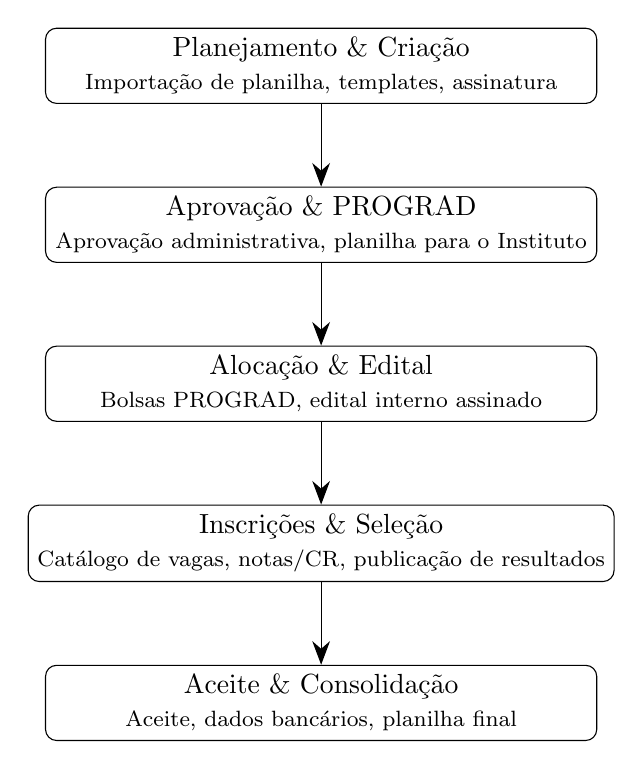
\begin{tikzpicture}[
    node distance=1.05cm,
    every node/.style={rounded corners, draw, align=center, minimum width=7cm, minimum height=0.82cm},
    >={Stealth[length=3mm]}
  ]
    \node (fase1) {Planejamento \& Criação\\\footnotesize Importação de planilha, templates, assinatura};
    \node[below=of fase1] (fase2) {Aprovação \& PROGRAD\\\footnotesize Aprovação administrativa, planilha para o Instituto};
    \node[below=of fase2] (fase3) {Alocação \& Edital\\\footnotesize Bolsas PROGRAD, edital interno assinado};
    \node[below=of fase3] (fase4) {Inscrições \& Seleção\\\footnotesize Catálogo de vagas, notas/CR, publicação de resultados};
    \node[below=of fase4] (fase5) {Aceite \& Consolidação\\\footnotesize Aceite, dados bancários, planilha final};

    \draw[->] (fase1) -- (fase2);
    \draw[->] (fase2) -- (fase3);
    \draw[->] (fase3) -- (fase4);
    \draw[->] (fase4) -- (fase5);
  \end{tikzpicture}
  \caption{Fluxo de processos do semestre de monitoria.}
  \label{fig:process-flow}
\end{figure}

Em \textit{Gerenciar Projetos}, o administrador acompanha submissões, aprovações e gera a planilha consolidada para o Instituto/PROGRAD, garantindo padronização e trilhas de auditoria.

\subsection{Implementação e Tecnologias}

O sistema foi implementado utilizando um conjunto coeso de tecnologias modernas e consolidadas, selecionadas para maximizar produtividade de desenvolvimento, segurança e manutenibilidade. No \textit{frontend}, adotou-se Next.js 15.1.4 com App Router, um framework React de produção que oferece renderização híbrida (SSR e CSR), otimizações automáticas de desempenho e roteamento baseado em sistema de arquivos. TypeScript 5.x foi utilizado em todo o código-fonte para garantir \textit{type safety} e detectar erros em tempo de desenvolvimento. A interface visual foi construída com Tailwind CSS, um framework utilitário que proporciona consistência e rapidez na estilização, complementado por shadcn/ui, uma coleção de componentes acessíveis e personalizáveis. Os formulários são implementados com React Hook Form, que minimiza re-renderizações desnecessárias e oferece validação eficiente, combinado com Zod para esquemas de validação compartilhados entre cliente e servidor. A sincronização de estado remoto e o gerenciamento de cache são tratados por React Query (TanStack Query), que automatiza requisições, invalidações e atualizações otimistas.

No \textit{backend}, a API foi construída com tRPC v11, uma solução inovadora que elimina a necessidade de definições duplicadas de tipos entre cliente e servidor, garantindo que toda comunicação seja completamente tipada em tempo de compilação. A autenticação e gerenciamento de sessões são realizados por Lucia Auth, um framework moderno que oferece flexibilidade e segurança superiores a soluções legadas. A persistência de dados utiliza Drizzle ORM em conjunto com PostgreSQL, proporcionando consultas SQL tipadas e migrações versionadas de forma declarativa. Para armazenamento de arquivos binários (históricos acadêmicos, documentos comprobatórios, PDFs gerados), o sistema emprega MinIO, uma solução compatível com o protocolo S3 da Amazon que facilita futuras migrações para serviços de nuvem. O envio automatizado de notificações por e-mail é realizado via Nodemailer, configurado para utilizar o servidor SMTP institucional da UFBA.

A infraestrutura de \textit{DevOps} foi projetada para garantir qualidade e confiabilidade através de práticas modernas de integração e entrega contínuas. A solução completa é containerizada com Docker, incluindo o banco de dados PostgreSQL, o servidor MinIO e a aplicação Node.js, facilitando implantação consistente em diferentes ambientes (desenvolvimento, homologação e produção). Uma pipeline automatizada no GitHub Actions executa validações a cada commit: linting e formatação de código com Biome, verificação estática de tipos com TypeScript, execução de testes unitários com Vitest para validar a lógica de negócio, execução de testes end-to-end com Playwright para validar fluxos completos do usuário, e build de produção para detectar erros de compilação antecipadamente. Essa abordagem garante que apenas código validado e livre de regressões seja promovido para ambientes de produção.

A organização da lógica de negócio segue uma estrutura modular baseada em routers tRPC especializados por domínio. O router principal (\texttt{appRouter}) agrega routers específicos para autenticação e usuários (\texttt{auth}, \texttt{me}, \texttt{user}, \texttt{apiKey}), entidades acadêmicas (\texttt{departamento}, \texttt{curso}, \texttt{discipline}), gestão de monitoria (\texttt{projeto}, \texttt{projetoTemplates}, \texttt{edital}, \texttt{inscricao}, \texttt{selecao}, \texttt{vagas}), funcionalidades administrativas (\texttt{importProjects}, \texttt{scholarshipAllocation}, \texttt{analytics}, \texttt{relatorios}) e infraestrutura transversal (\texttt{file}, \texttt{signature}, \texttt{notificacoes}). Essa separação facilita a compreensão do código, permite testes isolados de cada módulo e viabiliza o desenvolvimento paralelo por múltiplos desenvolvedores sem conflitos significativos.

\subsection{Interfaces do Sistema}

O sistema oferece interfaces especializadas para cada perfil de usuário. A página inicial (Figura \ref{fig:landing}) apresenta a proposta do sistema e acesso ao login institucional. O dashboard administrativo (Figura \ref{fig:dashboard}) consolida indicadores operacionais e oferece navegação rápida para tarefas críticas. A interface de assinatura (Figura \ref{fig:professor-assinatura}) permite que o professor visualize o PDF gerado e realize a assinatura digital antes da submissão. Por fim, a planilha PROGRAD (Figura \ref{fig:planilha-prograd}) consolida projetos aprovados para envio ao Instituto.

\begin{figure}[p]
  \centering
  \includegraphics[width=0.95\linewidth]{images/monitoria/landing.png}
  \caption{Página inicial pública do sistema.}
  \label{fig:landing}
\end{figure}

\begin{figure}[p]
  \centering
  \includegraphics[width=0.95\linewidth]{images/monitoria/admin-dashboard.png}
  \caption{Dashboard administrativo com métricas.}
  \label{fig:dashboard}
\end{figure}

\begin{figure}[p]
  \centering
  \includegraphics[width=0.95\linewidth]{images/Assinatura de Projeto.png}
  \caption{Assinatura de projeto pelo professor com prévia do PDF.}
  \label{fig:professor-assinatura}
\end{figure}

\begin{figure}[p]
  \centering
  \includegraphics[width=0.95\linewidth]{images/Planilha Prograd.png}
  \caption{Geração de planilha PROGRAD com projetos aprovados.}
  \label{fig:planilha-prograd}
\end{figure}

\section{Avaliação Experimental}
\label{sec:evaluation}

A avaliação do sistema combinou validação técnica e estudo qualitativo exploratório. Na dimensão técnica, 55 testes automatizados (unitários e de integração) em 15 arquivos cobrem fluxos críticos: controle de acesso RBAC, workflow de projetos, processo seletivo, importação de planejamento e publicação de editais. A taxa de sucesso foi de 100\% com tempo de execução de 1.07s para a suíte completa.

\subsection{Avaliação com Usuários}

Foi conduzida uma avaliação qualitativa com dois participantes representativos dos perfis prioritários do sistema: um administrador (coordenador de monitoria com cinco anos de experiência no processo) e um professor (docente ativo com histórico de participação em projetos de monitoria)~\cite{nielsen1994usability, lazar2017research}. A seleção priorizou usuários com conhecimento aprofundado do fluxo institucional vigente, permitindo comparação direta entre o processo manual atual e a solução proposta.

O foco da avaliação compreendeu o fluxo principal do sistema: importação de planejamento $\rightarrow$ templates $\rightarrow$ assinatura $\rightarrow$ aprovação $\rightarrow$ planilha PROGRAD. A metodologia combinou três técnicas complementares: \textit{walkthrough} guiado para observar a execução de tarefas específicas, protocolo \textit{think-aloud} para capturar percepções em tempo real, e entrevista semiestruturada para aprofundar pontos críticos. A análise dos dados seguiu o método de análise temática~\cite{braun2006using}, identificando padrões recorrentes nas verbalizações dos participantes.

Os principais achados foram organizados em três dimensões. Na dimensão de \textbf{usabilidade}, destacou-se a organização lógica do menu lateral, o onboarding claro com indicadores visuais de progresso, a pré-visualização de PDF antes da assinatura e o processo de assinatura digital intuitivo. O administrador observou que ``o sistema guia naturalmente para as próximas etapas'', enquanto o professor destacou a clareza dos estados de projeto (rascunho, submetido, aprovado).

Na dimensão de \textbf{utilidade}, os templates reutilizáveis foram avaliados como excelentes para economia de tempo, eliminando a necessidade de recriar projetos a cada semestre. A importação automática de planejamento foi considerada eficiente, e a planilha PROGRAD foi classificada como adequada para o trâmite institucional. O coordenador estimou redução de aproximadamente 70\% no tempo dedicado à consolidação de dados.

Na dimensão de \textbf{adoção}, ambos participantes confirmaram a viabilidade para uso em semestre real, condicionada a ajustes pontuais. As principais sugestões incluem: implementação de notificações por e-mail ao professor quando houver solicitação de ajustes, relocação do acesso à planilha PROGRAD para a seção de Projetos (maior proximidade conceitual), e inclusão de filtros avançados na listagem de projetos.

Do ponto de vista de \textbf{aprendizado}, os participantes relataram facilidade na compreensão do fluxo geral do sistema após breve orientação inicial. O coordenador destacou que a curva de aprendizado foi significativamente menor comparada a outros sistemas administrativos utilizados na universidade, atribuindo essa facilidade à interface consistente e aos feedbacks visuais claros em cada etapa. O professor mencionou que a documentação integrada (tooltips e mensagens de ajuda contextual) reduziu a necessidade de consultas externas durante a execução das tarefas.

Em termos de \textbf{confiabilidade percebida}, ambos participantes expressaram confiança na integridade dos dados processados pelo sistema. A geração automática de PDFs com assinatura digital foi especialmente valorizada por eliminar o risco de inconsistências entre versões de documentos. O coordenador ressaltou que a trilha de auditoria disponível no histórico de cada projeto oferece transparência e facilita a prestação de contas em eventuais auditorias institucionais, aspecto considerado crítico para adoção em ambiente de produção.

\subsection{Limitações}

O presente trabalho apresenta limitações metodológicas e de escopo que devem ser consideradas na interpretação dos resultados. Em relação à \textbf{amostra}, a avaliação qualitativa envolveu apenas dois participantes (N=2), o que limita a generalização dos achados para outros contextos institucionais. A ausência do perfil estudante na avaliação representa uma lacuna importante, dado que este grupo constitui parcela significativa dos usuários finais do sistema.

Quanto ao \textbf{ambiente de avaliação}, os testes foram conduzidos em ambiente local de desenvolvimento com variáveis de configuração específicas (banco de dados PostgreSQL local, servidor MinIO de desenvolvimento e credenciais de teste), o que pode não refletir completamente as condições de uso em produção, especialmente em períodos de alta demanda como abertura de inscrições. A ausência de métricas comparativas quantitativas (tempo médio por tarefa no processo manual versus sistema) impede a mensuração objetiva dos ganhos de eficiência.

Do ponto de vista de \textbf{validade externa}, há viés de seleção na amostra: os participantes possuem familiaridade tecnológica acima da média, o que pode ter favorecido a percepção positiva do sistema. Professores com menor afinidade tecnológica podem enfrentar curva de aprendizado mais acentuada. Adicionalmente, o sistema foi desenvolvido especificamente para o Instituto de Computação, e adaptações serão necessárias para expansão a outros departamentos com fluxos distintos.

Em relação às \textbf{limitações técnicas}, a integração com o sistema acadêmico institucional (SIAC) permanece parcial, exigindo que estudantes anexem documentos comprobatórios manualmente durante a inscrição ao invés de captura automática de históricos e notas. O módulo de relatórios finais e certificados (Fase 6 do fluxo de monitoria) foi especificado nos requisitos mas não implementado nesta versão, sendo priorizado como evolução futura. A ausência de testes de carga sistemáticos também representa uma limitação, dado que o comportamento do sistema sob uso concorrente intenso não foi avaliado experimentalmente.

Por fim, no que diz respeito às \textbf{limitações de escopo}, o sistema foi projetado para o contexto específico do Instituto de Computação da UFBA, incorporando regras de negócio e fluxos administrativos particulares desta unidade. A generalização para outros departamentos ou instituições demandará adaptações no modelo de dados, nas regras de validação e possivelmente na interface de usuário. A dependência de infraestrutura institucional (servidor SMTP da UFBA, domínio institucional para autenticação) também configura uma restrição para replicação imediata em outros contextos.


\FloatBarrier

\section{Conclusão e Trabalhos Futuros}
\label{sec:conclusion}

Este trabalho apresentou o Sistema de Monitoria-IC como solução para automatizar o \textit{workflow} de monitoria acadêmica. As contribuições centrais incluem: automação das etapas do processo (importação de planejamento, assinatura digital, aprovação administrativa e geração de planilhas PROGRAD), arquitetura moderna com separação de responsabilidades e base estruturada para futuras evoluções.

O principal desafio técnico foi a implementação da assinatura digital com sobreposição no PDF e integração com MinIO. Desafios organizacionais incluíram alinhamento de requisitos com stakeholders e adequação a procedimentos institucionais. Permanecem como limitações: integração parcial com sistema acadêmico (SIAC), escopo restrito ao IC e dependência de setores externos.

Trabalhos futuros contemplam: piloto institucional com métricas quantitativas de impacto, integração completa com SIAC, desenvolvimento de aplicativo móvel e expansão para outros departamentos. No longo prazo, busca-se disponibilizar o código como software livre para outras universidades. O código fonte está disponível em \url{https://github.com/luisfelipesena/sistema-de-monitoria-ic} e o sistema em \url{https://sistema-de-monitoria.app.ic.ufba.br/}.

\FloatBarrier

\section*{Agradecimentos}

Agradeço ao Instituto de Computação da UFBA pelo apoio institucional, aos professores e alunos que participaram dos testes piloto, e à equipe de TI que viabilizou a infraestrutura necessária.

\bibliographystyle{apalike-sol}
\bibliography{references}

\end{document}